% Shared standalone design for the editable figure reconstructions.
\documentclass[tikz,border=5pt,10pt]{standalone}
\usepackage[T1]{fontenc}
\usepackage[utf8]{inputenc}
\usepackage{newpxtext,newpxmath}
\usepackage[scaled=.94]{sourcesanspro}
\usepackage{pgfplots}
\pgfplotsset{compat=1.18}
\usetikzlibrary{arrows.meta,calc,positioning,decorations.pathreplacing,
  decorations.markings,patterns,matrix,shapes.geometric,fit,backgrounds,
  intersections,angles,quotes}
\definecolor{ink}{HTML}{203746}
\definecolor{accent}{HTML}{146C78}
\definecolor{muted}{HTML}{667780}
\definecolor{signalred}{HTML}{B94B44}
\color{ink}
\tikzset{>=Latex,line width=.8pt,
  every node/.style={font=\small},
  axis/.style={->,draw=muted,line width=.5pt},
  guide/.style={draw=muted,dashed,line width=.45pt},
  curve/.style={draw=accent,line width=1pt},
  marker/.style={circle,fill=accent,inner sep=1.5pt},
  labelbox/.style={fill=white,inner sep=2pt}}

\begin{document}
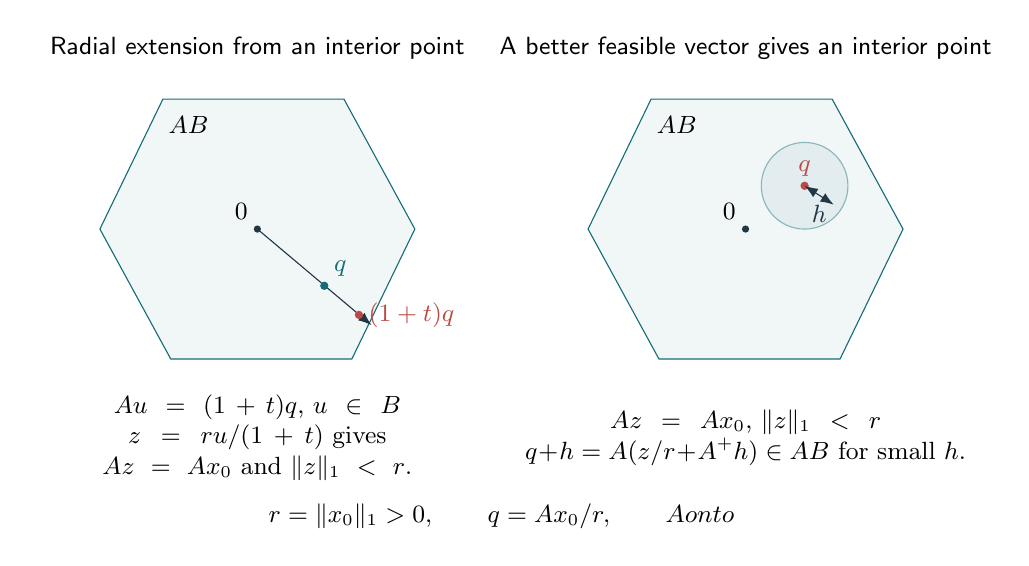
\begin{tikzpicture}
\foreach \s in {0,6.2}{\begin{scope}[shift={(\s,0)}]
\path[draw=accent,fill=accent!6](-2,0)--(-1.2,1.65)--(1.1,1.65)--(2,0)--(1.2,-1.65)--(-1.1,-1.65)--cycle;
\node[anchor=north west]at(-1.25,1.55){$AB$};\fill[ink](0,0)circle(1.3pt);\node[above left]at(0,0){$0$};
\end{scope}}
\node[font=\small\sffamily]at(0,2.3){Radial extension from an interior point};
\draw[->,ink](0,0)--(1.45,-1.22);
\fill[accent](.85,-.72)circle(1.5pt)node[above right]{$q$};
\fill[signalred](1.29,-1.09)circle(1.5pt)node[right]{$(1+t)q$};
\node[align=center,text width=5.6cm]at(0,-2.65){$Au=(1+t)q$, $u\in B$\\$z=ru/(1+t)$ gives $Az=Ax_0$ and $\|z\|_1<r$.};
\node[font=\small\sffamily]at(6.2,2.3){A better feasible vector gives an interior point};
\draw[accent!50,fill=accent!12](6.95,.55)circle(.55);
\fill[signalred](6.95,.55)circle(1.5pt)node[above]{$q$};
\draw[<->,ink](6.95,.55)--(7.32,.31)node[midway,below]{$h$};
\node[align=center,text width=5.6cm]at(6.2,-2.65){$Az=Ax_0$, $\|z\|_1<r$\\$q+h=A(z/r+A^+h)\in AB$ for small $h$.};
\node at(3.1,-3.65){$r=\|x_0\|_1>0,\qquad q=Ax_0/r,\qquad A\text{ onto}$};
\end{tikzpicture}
\end{document}
